% To je predloga za poročila o domačih nalogah pri predmetih, katerih
% nosilec je Tomaž Curk. Avtor predloge je Blaž Zupan.
%
% Seveda lahko tudi dodaš kakšen nov, zanimiv in uporaben element,
% ki ga v tej predlogi (še) ni. Več o LaTeX-u izveš na
% spletu, na primer na http://tobi.oetiker.ch/lshort/lshort.pdf.%
% To predlogo lahko spremeniš v PDF dokument s pomočjo programa
% pdflatex, ki je del standardne instalacije LaTeX programov.

\documentclass[a4paper,11pt]{article}
\usepackage{a4wide}
\usepackage{fullpage}
\usepackage[utf8x]{inputenc}
\usepackage[english]{babel}
\selectlanguage{english}
\usepackage[toc,page]{appendix}
\usepackage[pdftex]{graphicx} % za slike
\usepackage{setspace}
\usepackage{color}
\definecolor{light-gray}{gray}{0.95}
\usepackage{listings}
\lstset{
  basicstyle=\ttfamily,
  columns=fullflexible,
  frame=single,
  breaklines=true,
  postbreak=\mbox{\textcolor{red}{$\hookrightarrow$}\space},
}
\usepackage{hyperref}
\renewcommand{\baselinestretch}{1.2} % za boljšo berljivost večji razmak
\renewcommand{\appendixpagename}{Appendix}

\lstset{ % nastavitve za izpis kode, sem lahko tudi kaj dodaš/spremeniš
language=Python,
basicstyle=\footnotesize,
basicstyle=\ttfamily\footnotesize\setstretch{1},
backgroundcolor=\color{light-gray},
}

\title{%
Analysis of song lyrics to match genre \\
\large Assignment 1: Basic text processing}
\author{Jernej Janež (63130077), Rok Marinšek (63130146), Luka Podgoršek (63130189)}
\date{\today}

\begin{document}

\maketitle

\section{NLP task}
% A paragraph of an NLP task/idea that you solved. A short description of your solution and related work in the field.
For our assignment we decided to analyze song lyrics, extract keywords that correspond to specific genres and try to classify song by its lyrics to corresponding genre. First we found a \href{https://www.kaggle.com/gyani95/380000-lyrics-from-metrolyrics}{dataset} that cointained song lyrics. We preprocessed data, trained and tested a model and presented results with graphs. Some similar solutions already exist but perform similar task with neural networks or some other more complex methods. With this assignment we wanted to find out if our aproach can provide satisfactory results by using simple natural language processing techniques.

\section{Data}
% A description of (train, development, test) data or its retrieval
% Also describe metrics, used to score the performance of your algorithms.
We searched the internet for appropriate dataset. We found many different but in the end decided to use \href{https://www.kaggle.com/gyani95/380000-lyrics-from-metrolyrics}{\textit{380,000+ lyrics from MetroLyrics dataset}} found on kaggle portal. This dataset had the attributes we needed to solve our task.

\noindent Dataset contained following attributes:
\begin{itemize}
\item song title,
\item year,
\item artist
\item genre,
\item lyrics.
\end{itemize}

\subsection{Data preparation}
Data we found was stored in \textit{.csv} file. Because it contained more than \textit{380 000} entries we decided to analyze songs that we're released in 2016 (latest songs in dataset). Afterwards we filtered songs to match predefind genres. We selected \textit{hip-hop, pop  and metal} and ended up with \textit{6845} different songs. Then we removed lyrics that we're shorter than 100 words and longer than 1000 words. This way we removed outliers in data.

When we finished data preparation and selection we focused on the text preparation. First we removed special characters from text with regular expressions, converted words to lowercase and removed punctuations. Finally we removed non-english songs. This way we ended up with \textbf{5613} different songs.

\begin{table}[h!]
\centering
\label{baseline}
\begin{tabular}{clc}
\hline
\# & Genre & Number of different songs \\
\hline
0 & Hip-Hop & 2180 \\
1 & Metal & 814 \\
2 & Pop & 2619 \\
\end{tabular}
\caption{Number of songs per genre}
\end{table}

In the end we saved filtered data into \textit{.csv} file. In our model class we used this file as input to train our model. You can also use this file to replicate our results.

\section{Model}

To train our model we used preprocessed file. Model is build with logistic regression.

\subsection{Train, test data and metrics}
% 80 20, regressing 0.2
% A description of (train, development, test) data or its retrieval. Also describe metrics, used to score the performance of your algorithms.
To train our model we used 80\% of data and 20\% to test our model. To measure score and performance of our model we used following metrics:
\begin{itemize}
\item accuracy,
\item precision,
\item recall,
\item and f1 score.
\end{itemize}

In development phase we also played with regularization factor. We used above mentioned metrics to determine best regularization factor. In the end we set it to 1 (TODO UPDATE TO PROPER VALUE).

\subsection{Resources, tools and corpora}
%A description of tools and resources used. A list of additional linguistic corpora and how it was used to improve results of your algorithm

We used several different python libraries. Pandas was used for data structures and data purging. Nltk corpus was used to determine stopwords and for lematization. Langdetect library was used to remove non-english lyrics. To build our model we used sklearn and preseted results with matplotlib.

\section{Algorithm-Model description}
% describe how we build our model

% we used l regression-.....

\subsection{Building bag of words with TF-IDF}
Bag of words is an algorithm that counts how many times a word appears in a document. We used WhitespaceTokenizer function from the ntlk library to tokenize our song lyrics and removed all the stop words, because words such as \textit{"and"} or \textit{"the"} appear frequently in all songs and are systematically discounted. Then we used the WordNetLemmatizer function also from the nltk library to lemmatize the text which grouped together the different inflected forms of a word so they can be analyzed as a single item. After that we vectorized our data with TF-IDF function called TfidfVectorizer from sklearn which measured the number of times words appeared in a given song (term frequency). The more songs a word appears in, the less valuable that word is as a signal. That’s intended to leave only the frequent AND distinctive words as markers. Each word’s TF-IDF relevance is a normalized data format that also adds up to one.

\pagebreak
\section{Results}
% interpretacija modela, kaj je primerom skupno, zakaj pride do napačne klasifikacije

Before we could interprete our model and it's predictions we had to test it. Testing phase consisted of 10 iterations. In each iteration we sampled data with different random seed, trained a model and tested it on sampled test data. In the end we averaged all metrics to score performance of our model. You can find results in \hyperref[label-model-score]{table} bellow.

\begin{table}[h!]
\centering
\label{baseline}
\begin{tabular}{cccc}
\hline
Accuracy & Precision & recall & f1 \\
\hline
0.736 & 0.769 & 0.736 & 0.745 \\
\end{tabular}
\label{label-model-score}
\caption{Model scores}
\end{table}

\noindent Beside performance scores our model returned list of keywords that have the most and the least value for classification. These results are presented in tables bellow. Graphical presetation of tables is included in appendix \hyperref[label-graphs]{graphs section.}


\subsection{Postagging}
%top nouns and adjectives per genre

% slabosti modela
\subsection{Understanding wrong classifications}

If you look at confusion matrix

\begin{table}[h!]
\centering
\label{baseline}
\begin{tabular}{cccc}
\hline
+ Keywords & Weight & - Keywords & Weight \\
\hline
love & 1.60 & nigga & -2.95 \\
heart & 1.46 & shit & -2.17 \\
good & 1.28 & fuck & -2.15 \\
oh & 1.21 & bitch & -2.00 \\
miss & 1.18 & end & -1.84 \\
boy & 1.17 & dead & -1.59 \\
hurt & 1.07 & hell & -1.44 \\
blue & 1.03 & death & -1.38 \\
hey & 1.02 & die & -1.20 \\
goodbye & 1.00 & yo & -1.19 \\
\end{tabular}
\caption{Keywords for pop}
\end{table}

\begin{table}[h!]
\centering
\label{baseline}
\begin{tabular}{cccc}
\hline
+ Keywords & Weight & - Keywords & Weight \\
\hline
end & 2.46 & love & -2.49 \\
dead & 2.18 & like & -2.19 \\
hell & 1.77 & got & -2.01 \\
death & 1.76 & ain't & -1.99 \\
nothing & 1.65 & baby & -1.81 \\
fear & 1.52 & yeah & -1.77 \\
lie & 1.50 & nigga & -1.48 \\
eye & 1.45 & good & -1.39 \\
die & 1.38 & boy & -1.35 \\
memory & 1.37 & girl & -1.32 \\
\end{tabular}
\caption{Keywords for metal}
\end{table}

\begin{table}[h!]
\centering
\label{baseline}
\begin{tabular}{cccc}
\hline
+ Keywords & Weight & - Keywords & Weight \\
\hline
nigga & 4.42 & nothing & -1.36 \\
ain't & 2.92 & forget & -1.32 \\
bitch & 2.34 & world & -1.21 \\
shit & 2.13 & i've & -1.13 \\
got & 2.11 & angel & -0.97 \\
fuck & 1.99 & believe & -0.95 \\
gon' & 1.87 & light & -0.95 \\
like & 1.81 & memory & -0.90 \\
money & 1.66 & we'll & -0.89 \\
man & 1.54 & care & -0.88 \\
\end{tabular}
\caption{Keywords for hip-hop}
\end{table}


%\begin{table}[h!]
%\centering
%\label{baseline}
%\begin{tabular}{cccc}
%\end{tabular}
%\caption{Keywords for hip-hop}
%\end{table}

\pagebreak
\section{Github repository}
Github repository: \href{https://github.com/marok39/onj-02}{https://github.com/marok39/onj-02}


\appendix
\appendixpage
\section{\label{label-graphs} Graphs}

Here you can find visualization of all results. These files can be found alongside report in /img directory.

\begin{figure}[h]
\begin{center}
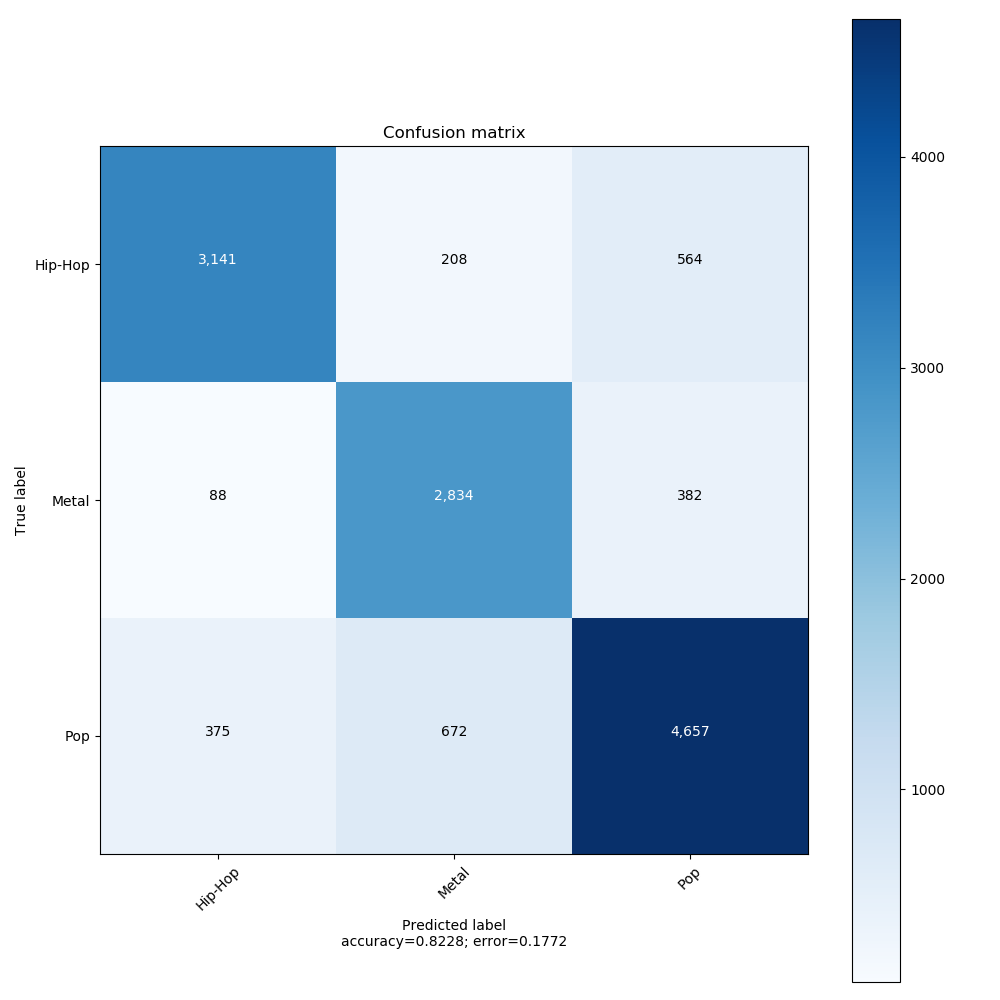
\includegraphics[width=0.8\textwidth]{./img/matrix.png}
\end{center}
\caption{Confisuin matrix}
\label{label-cf-matrix}
\end{figure}

\begin{figure}[h]
\begin{center}
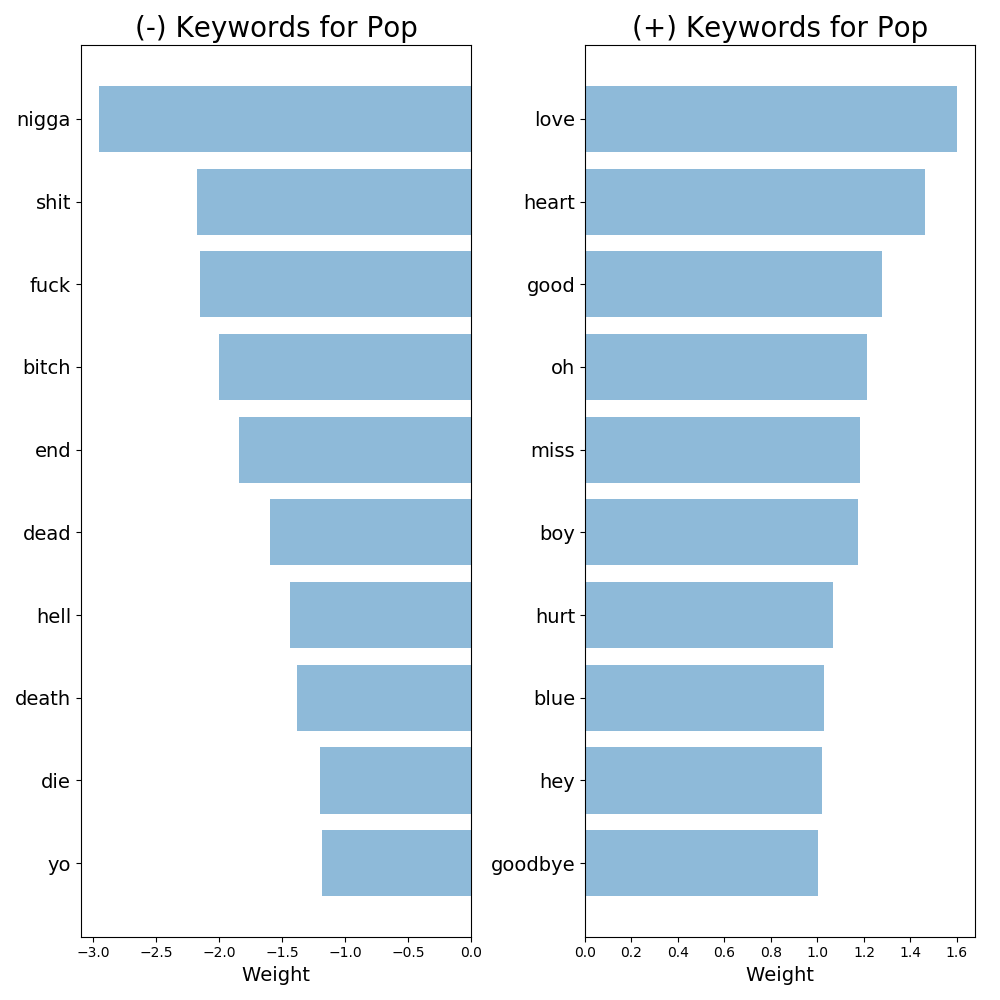
\includegraphics[width=0.8\textwidth]{./img/pop-keywords.png}
\end{center}
\caption{Keywords visualization for pop}
\label{label-kw-pop}
\end{figure}

\begin{figure}[h]
\begin{center}
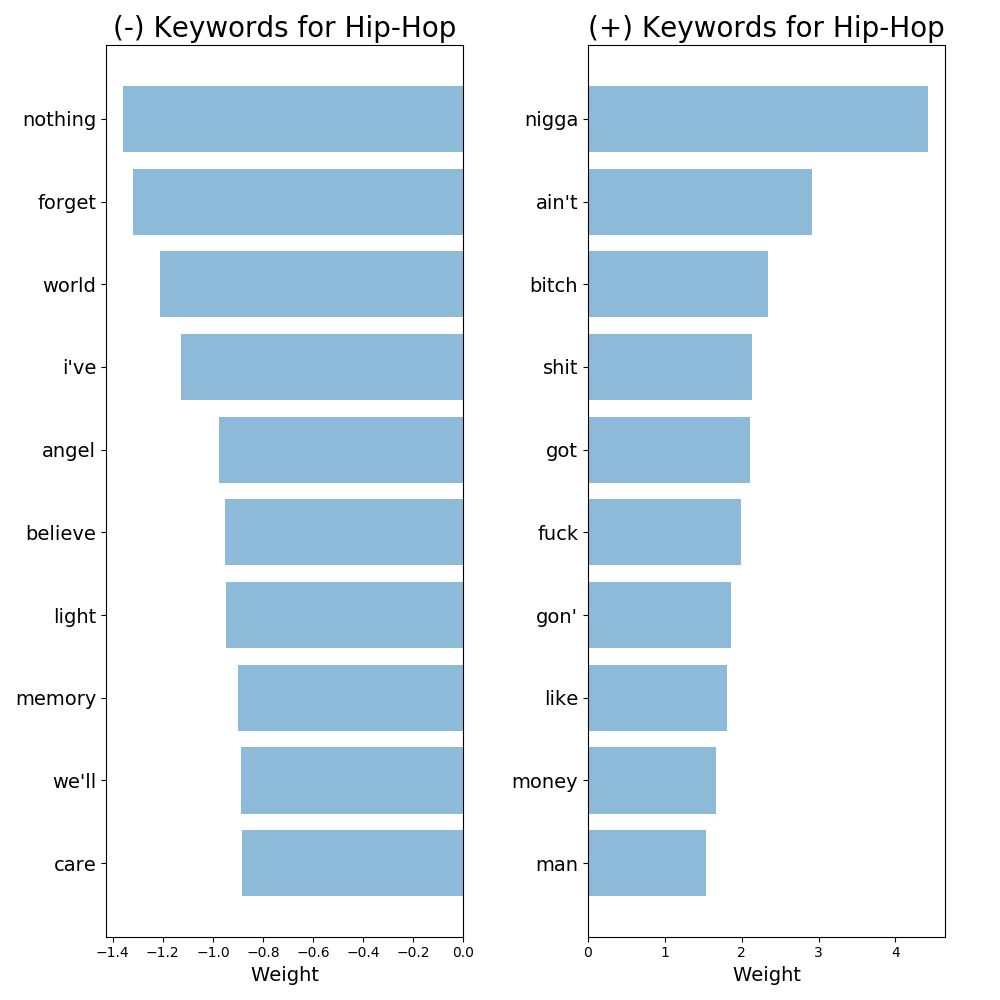
\includegraphics[width=0.8\textwidth]{./img/hip-hop-keywords.png}
\end{center}
\caption{Keywords visualization for hip-hop}
\label{label-kw-hip-hop}
\end{figure}

\begin{figure}[h]
\begin{center}
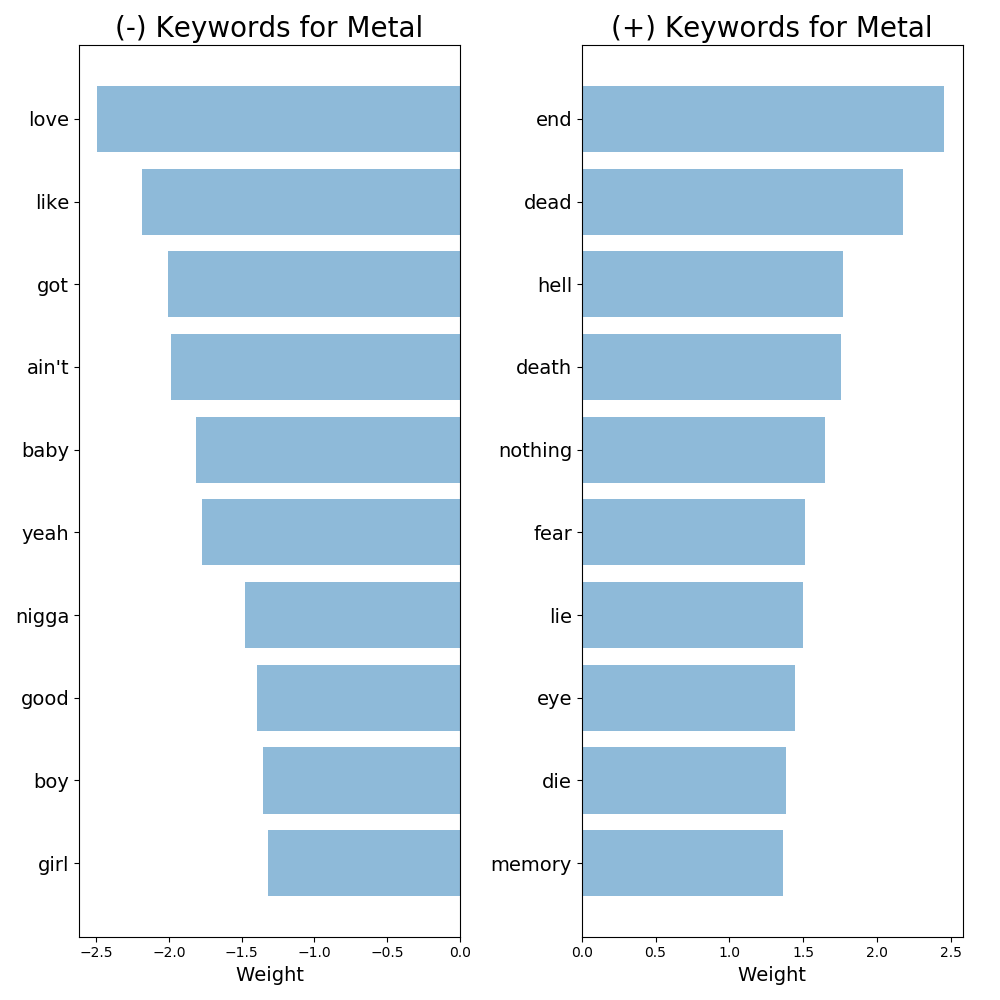
\includegraphics[width=0.8\textwidth]{./img/metal-keywords.png}
\end{center}
\caption{Keywords visualization for metal}
\label{label-kw-metal}
\end{figure}

%\begin{lstlisting}
%# comment
%\end{lstlisting}


\end{document}
